\chapter{系统设计}

\section{需求分析}

本视频编辑系统的需求分析基于技术可行性研究,主要涵盖功能性需求、
非功能性需求、技术约束和用户场景等方面。

在功能性需求方面,首先,多模态视频编辑功能应支持文本指令驱动、
参考图像风格迁移、虚拟换装和光照调整等多种编辑方式。其次,考虑到编辑过程需要预处理以及多轮训练,
系统无法实时的生成结果,因此需要在结果生成后告知用户。最后,作为实验室算法的展示平台,系统需要
具备一定的扩展性,以便于后续的算法更新和功能扩展。

非功能性需求方面,系统需要具备较高的安全性,应当采取的措施包括用户认证、数据库信息加密、前后端分离、
API接口鉴权等。此外,系统应该具有较好的可维护性,包括代码规范、模块化设计、应用文档编写等,以方便后续的维护和升级。

技术约束方面,系统部署在实验室服务器上,配置了cuda12.1与小规模计算平台,运算资源有限;同时由于部署在学校内网无法
直接通过外网访问,需要网络地址转换(NAT)技术提供访问支持。

用户场景方面,一方面该系统面向对最新人工智能技术感兴趣的研究者及普通用户,需要提供简洁易用的界面和友好的交互体验;
另方面该系统面向实验室研究者,为他们提供了解用户真实需求的渠道,需要提供相关的数据统计和分析功能。

\section{功能设计}

\subsection{用例设计}

一般用户在登录后可以上传视频并进行编辑、查询与管理编辑结果,并且可以查看开发者的相关信息。用户用例图如\ref{fig:user_uml}所示。
\begin{figure}[ht]
    \centering
    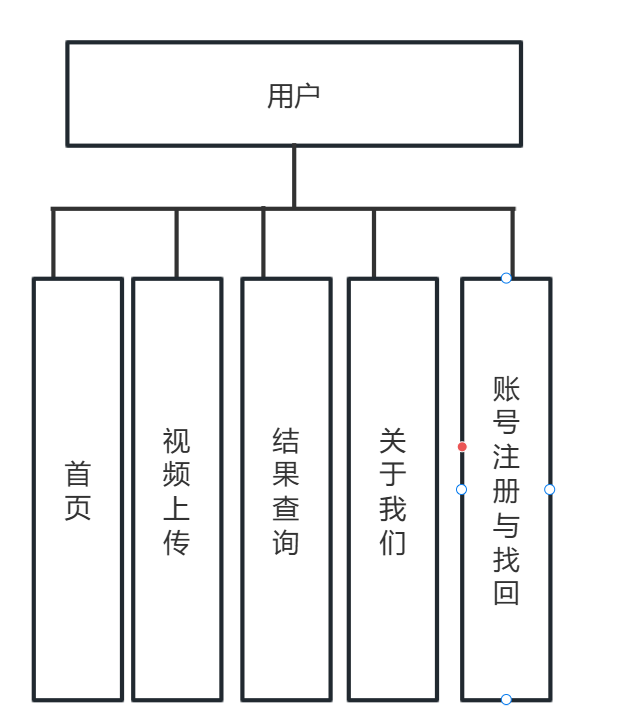
\includegraphics[width=0.3\textwidth]{source/img/user_uml.png}
    \bicaption{用户用例图}{User Use Case Diagram}
    \label{fig:user_uml}
\end{figure}
管理员用户除了一般用户所拥有的功能之外,还添加了数据统计与任务请求导出功能,以方便实验室研究者了解用户真实需求。管理员用户用例图如\ref{fig:admin_uml}所示。
\begin{figure}[ht]
    \centering
    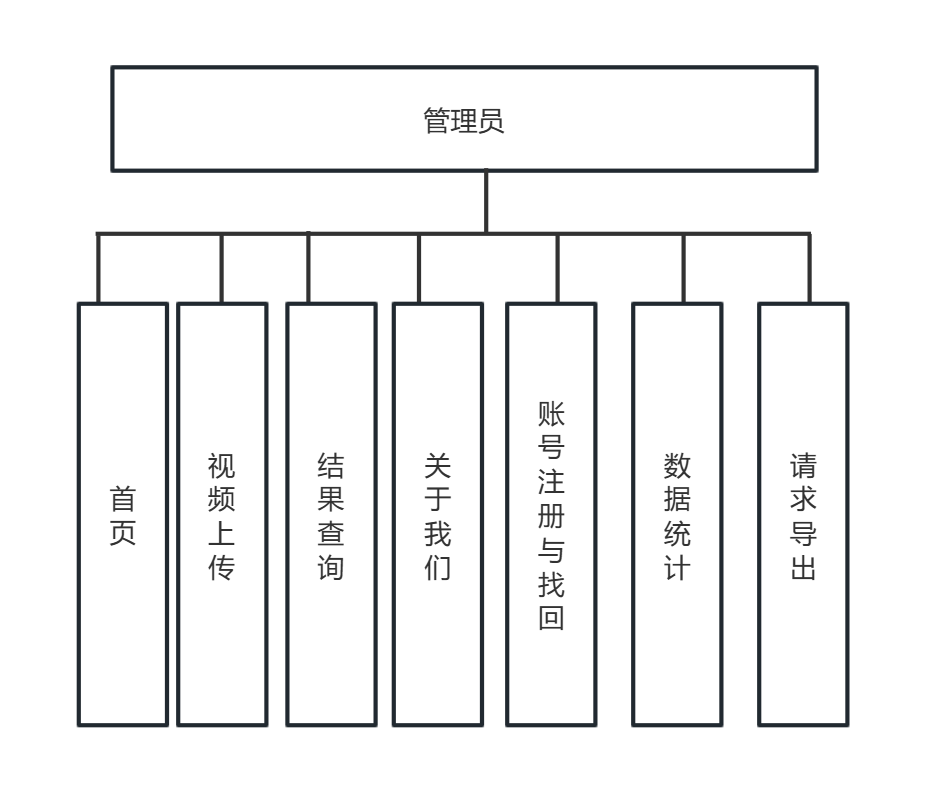
\includegraphics[width=0.4\textwidth]{source/img/admin_uml.png}
    \bicaption{管理员用例图}{Admin Use Case Diagram}
    \label{fig:admin_uml}
\end{figure}

\subsection{流程设计}

系统涉及到的工作流程主要包括登陆管理、任务上传与结果管理。

\subsubsection{登录管理}

由于用户的编辑结果通过邮箱来发送,我们可以将邮箱作为用户的唯一标识,在用户注册时将邮箱作为用户名,密码作为用户密码,通过邮箱和密码进行登录。
用户忘记密码时也可以通过邮箱进行密码重置。登录流程如\ref{fig:login_process}所示。
\begin{figure}[ht]
    \centering
    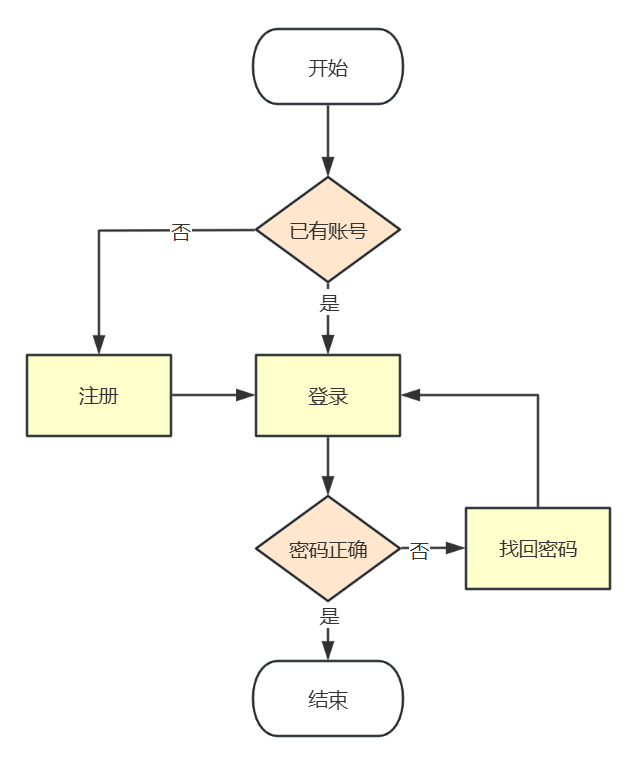
\includegraphics[width=0.4\textwidth]{source/img/login_process.png}
    \bicaption{登录流程图}{Login Process}
    \label{fig:login_process}
\end{figure}

\subsubsection{任务上传}

根据视频编辑算法的输入,需要用户提供视频、编辑提示类型与对应的提示内容,并提供邮箱以获取编辑结果。上传流程如\ref{fig:upload_process}所示。
\begin{figure}[ht]
    \centering
    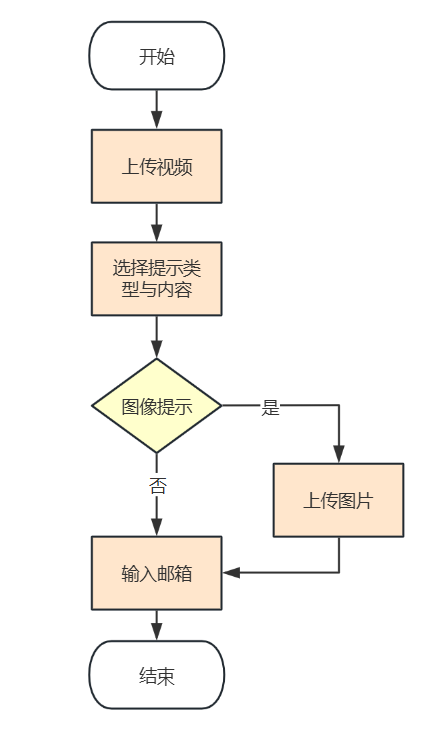
\includegraphics[width=0.3\textwidth]{source/img/edit_process.png}
    \bicaption{上传流程图}{Upload Process}
    \label{fig:upload_process}
\end{figure}

\subsubsection{结果管理}

用户在结果查询界面可以查看自己上传的任务进度与结果,系统也支持任务重命名与删除,同时在任务处理完成后会自动生成略缩图,方便用户预览结果。

\section{安全性设计}

在系统构建的过程中,安全性是一个至关重要的方面。为了防止未经授权的访问和操作,我们需要用户在登录状态下进行操作,这涉及到对用户信息与数据的
加密保护;我们也需要限制用户的操作行为,以防止用户的恶意操作;另外为了保证服务器的安全性,我们也需要系统部署过程中的安全措施。

\subsection{用户信息与数据加密}

我们将用户信息存储在

